\chapter{Appendix}

\noindent\textbf{Head-wise Similarity Analysis}

\begin{figure}[H]
    \centering
    \begin{subfigure}[t]{0.66\textwidth}
        \centering
        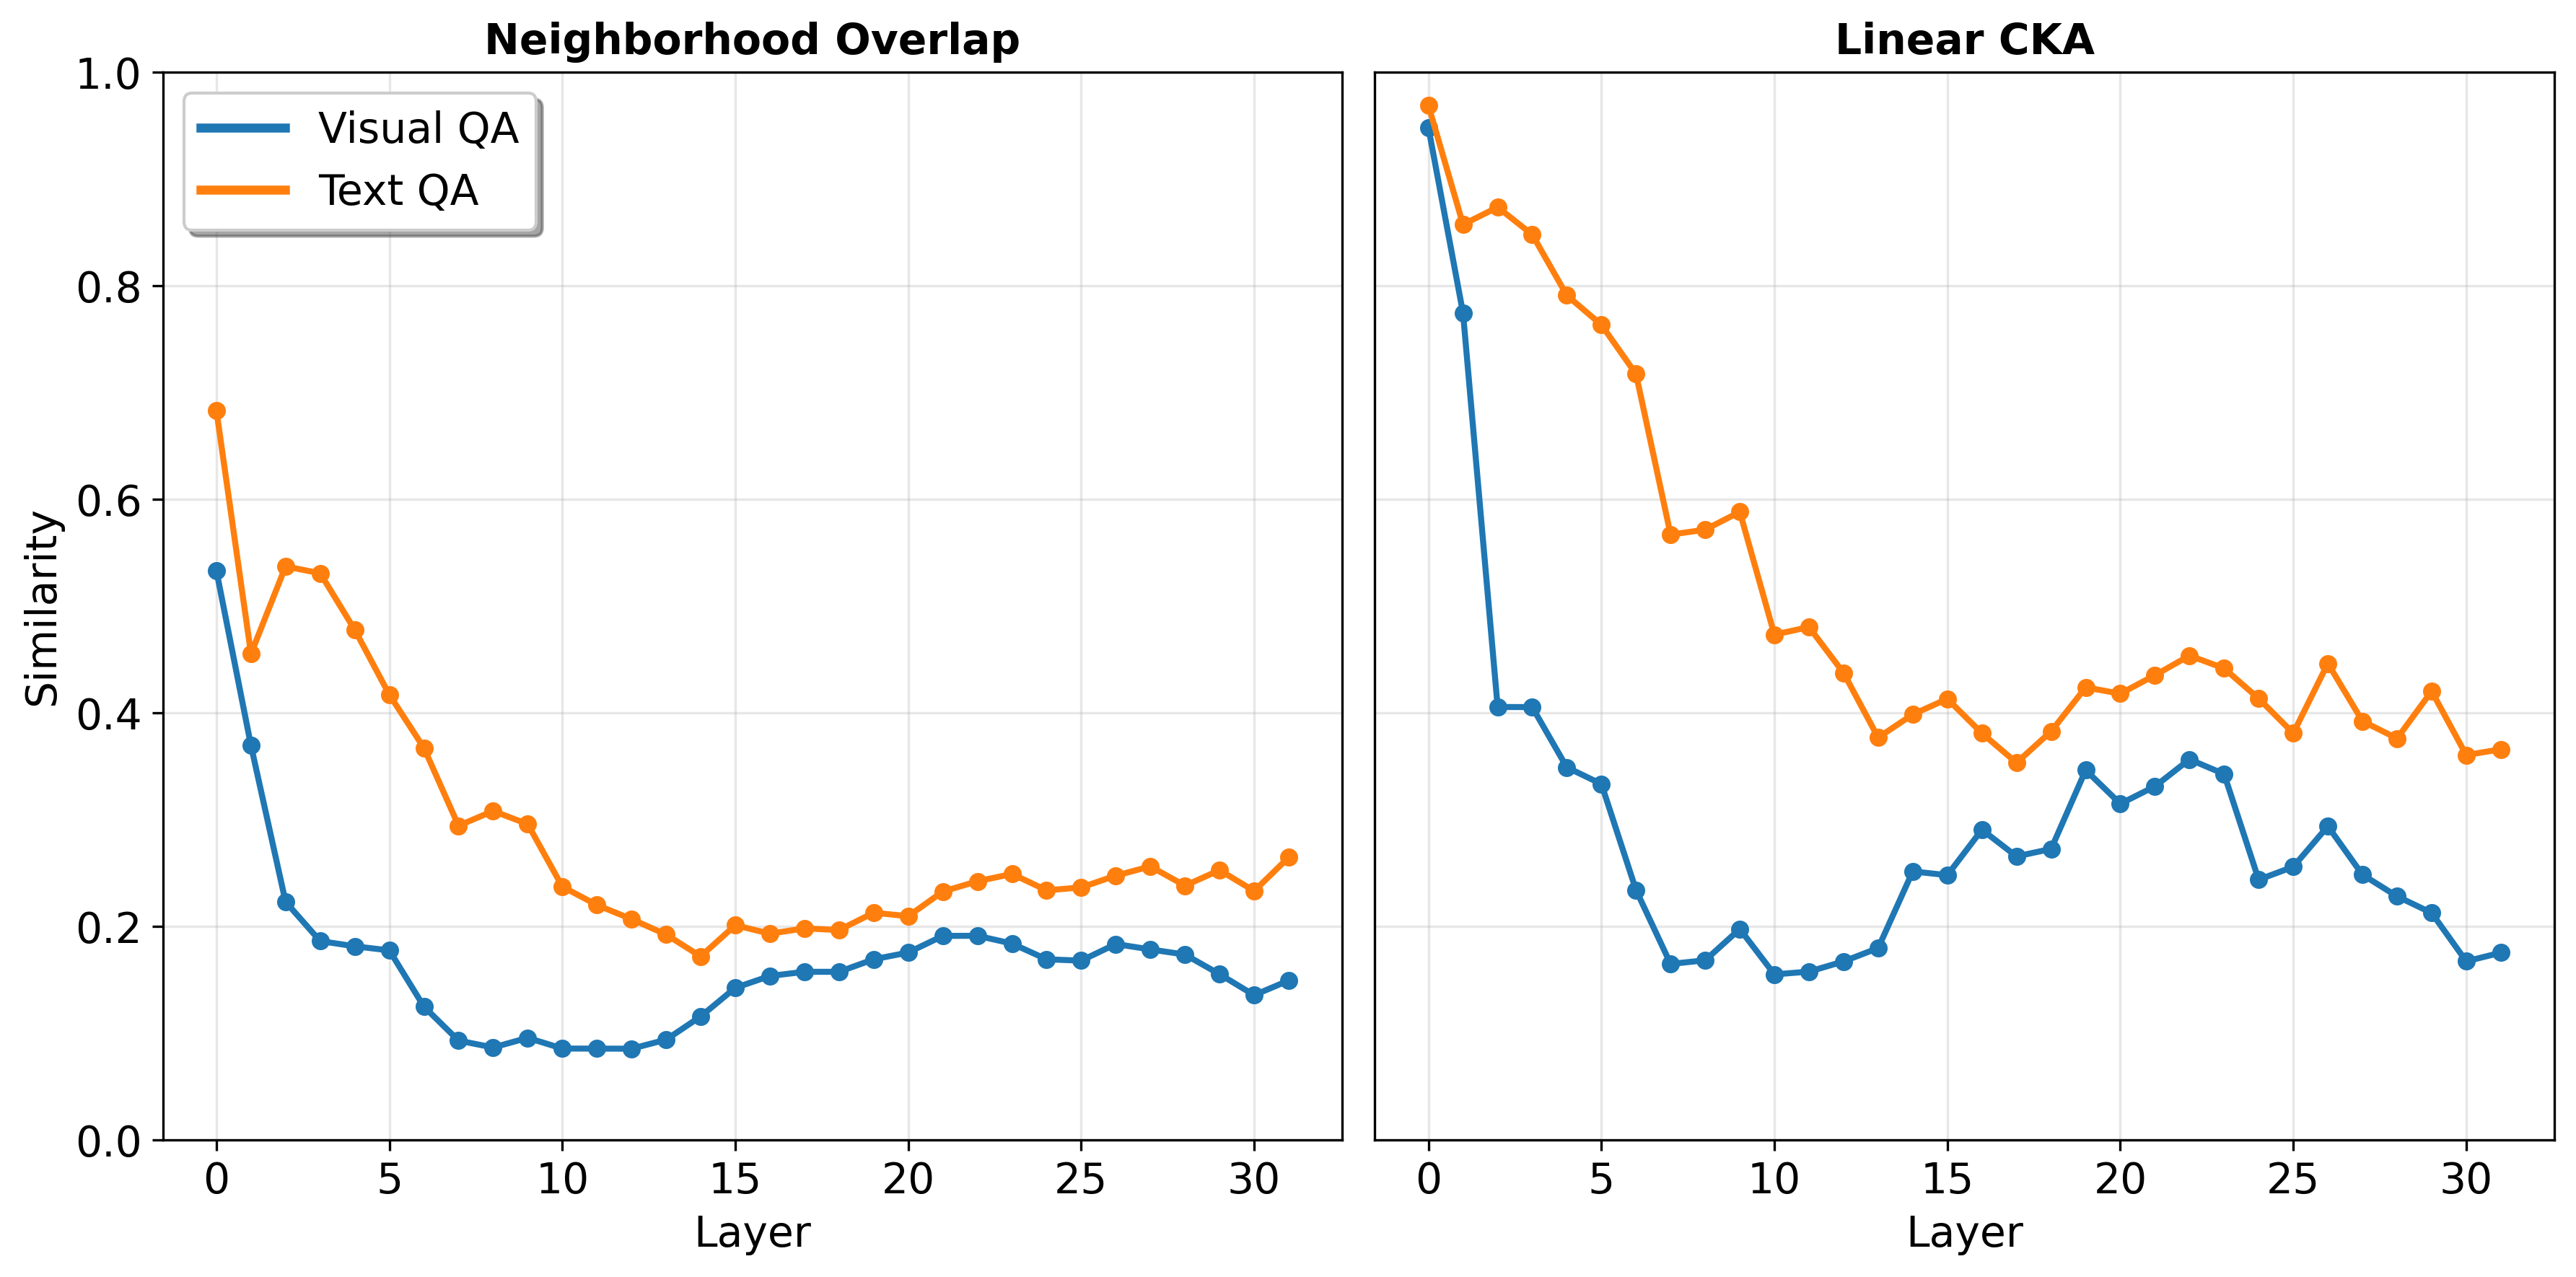
\includegraphics[width=\textwidth]{../images/chapter3/similarity_measures_mean_heads_projection_last_neighborhood_overlap_linear_cka.png}
        \vspace{-0.65cm}
        \caption{}
        \label{fig:layer_wise_similarity_cocovqa_mean_heads_combined}
    \end{subfigure}
    \begin{subfigure}[t]{0.33\textwidth}
        \centering
        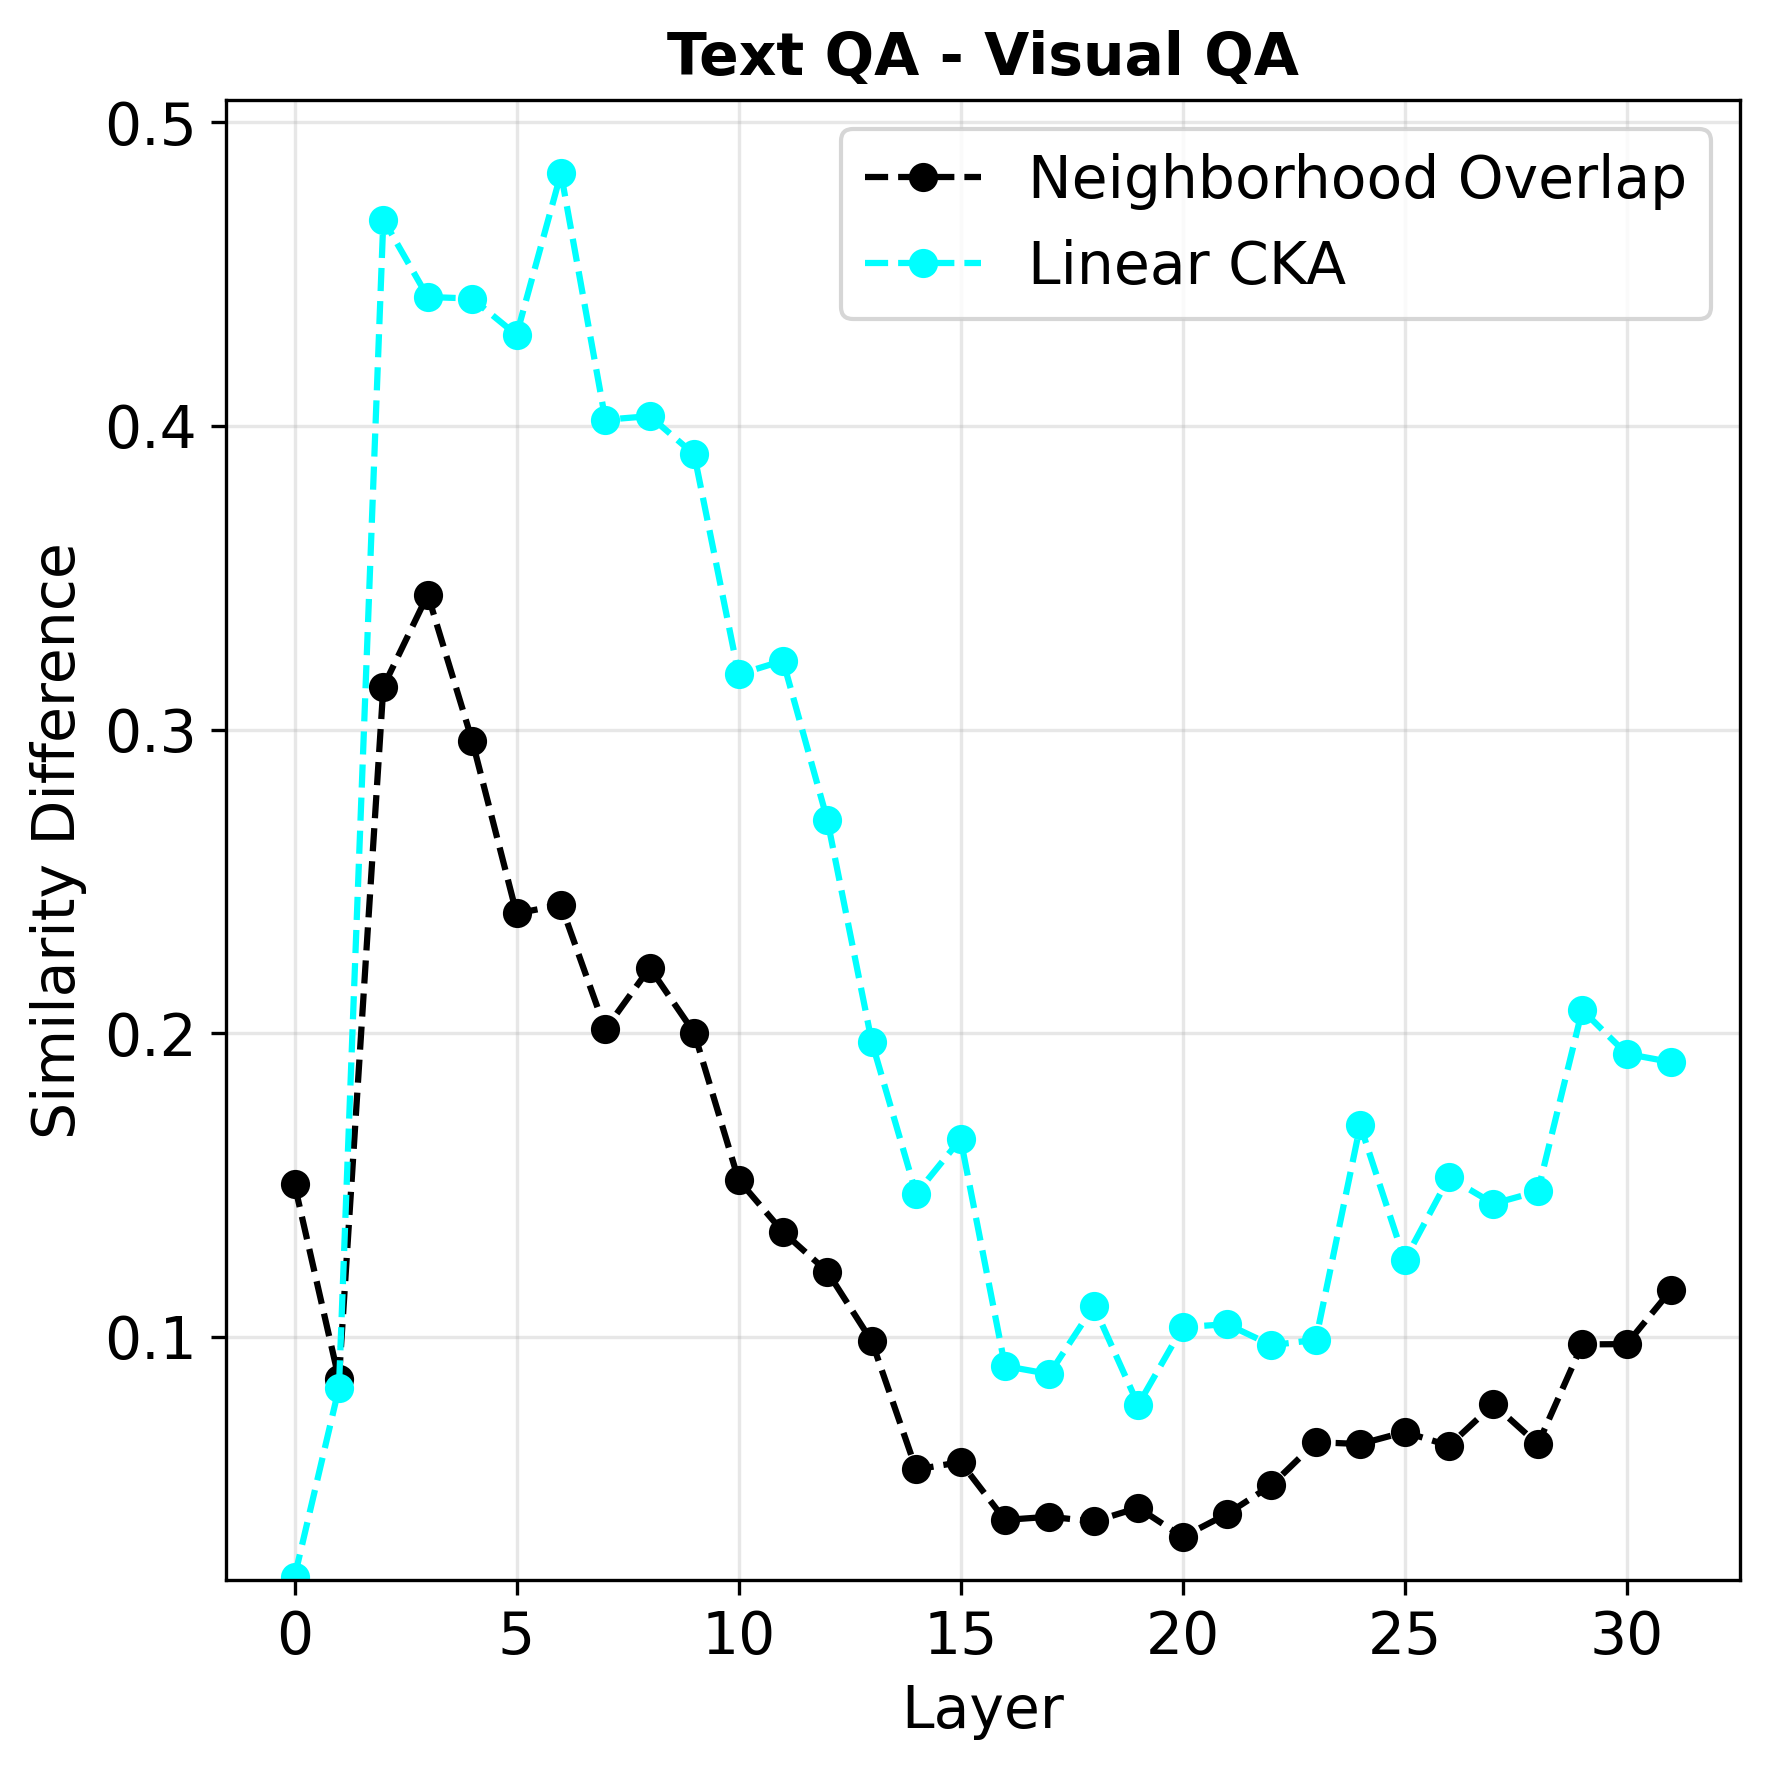
\includegraphics[width=\textwidth]{../images/chapter3/similarity_difference_measures_mean_heads_projection_last.png}
        \vspace{-0.65cm}
        \caption{}
        \label{fig:layer_wise_similarity_cocovqa_mean_heads_difference}
    \end{subfigure}
    \vspace{-0.3cm}
    \caption{
      Similar to Figure \ref{fig:layer_wise_similarity_cocovqa} but the values are the mean of the head-wise neighborhood overlap matrices of the text and multimodal similarites in Figure~\ref{fig:heads_wise_similarity_cocovqa}.
    }
    \label{fig:layer_wise_similarity_cocovqa_mean_heads}
\end{figure}

\newpage

\noindent\textbf{Dataset Entropy as a Measure of Data Representations Compactness}

\begin{figure}[H]
    \centering
    \begin{subfigure}[t]{0.65\textwidth}
        \centering
        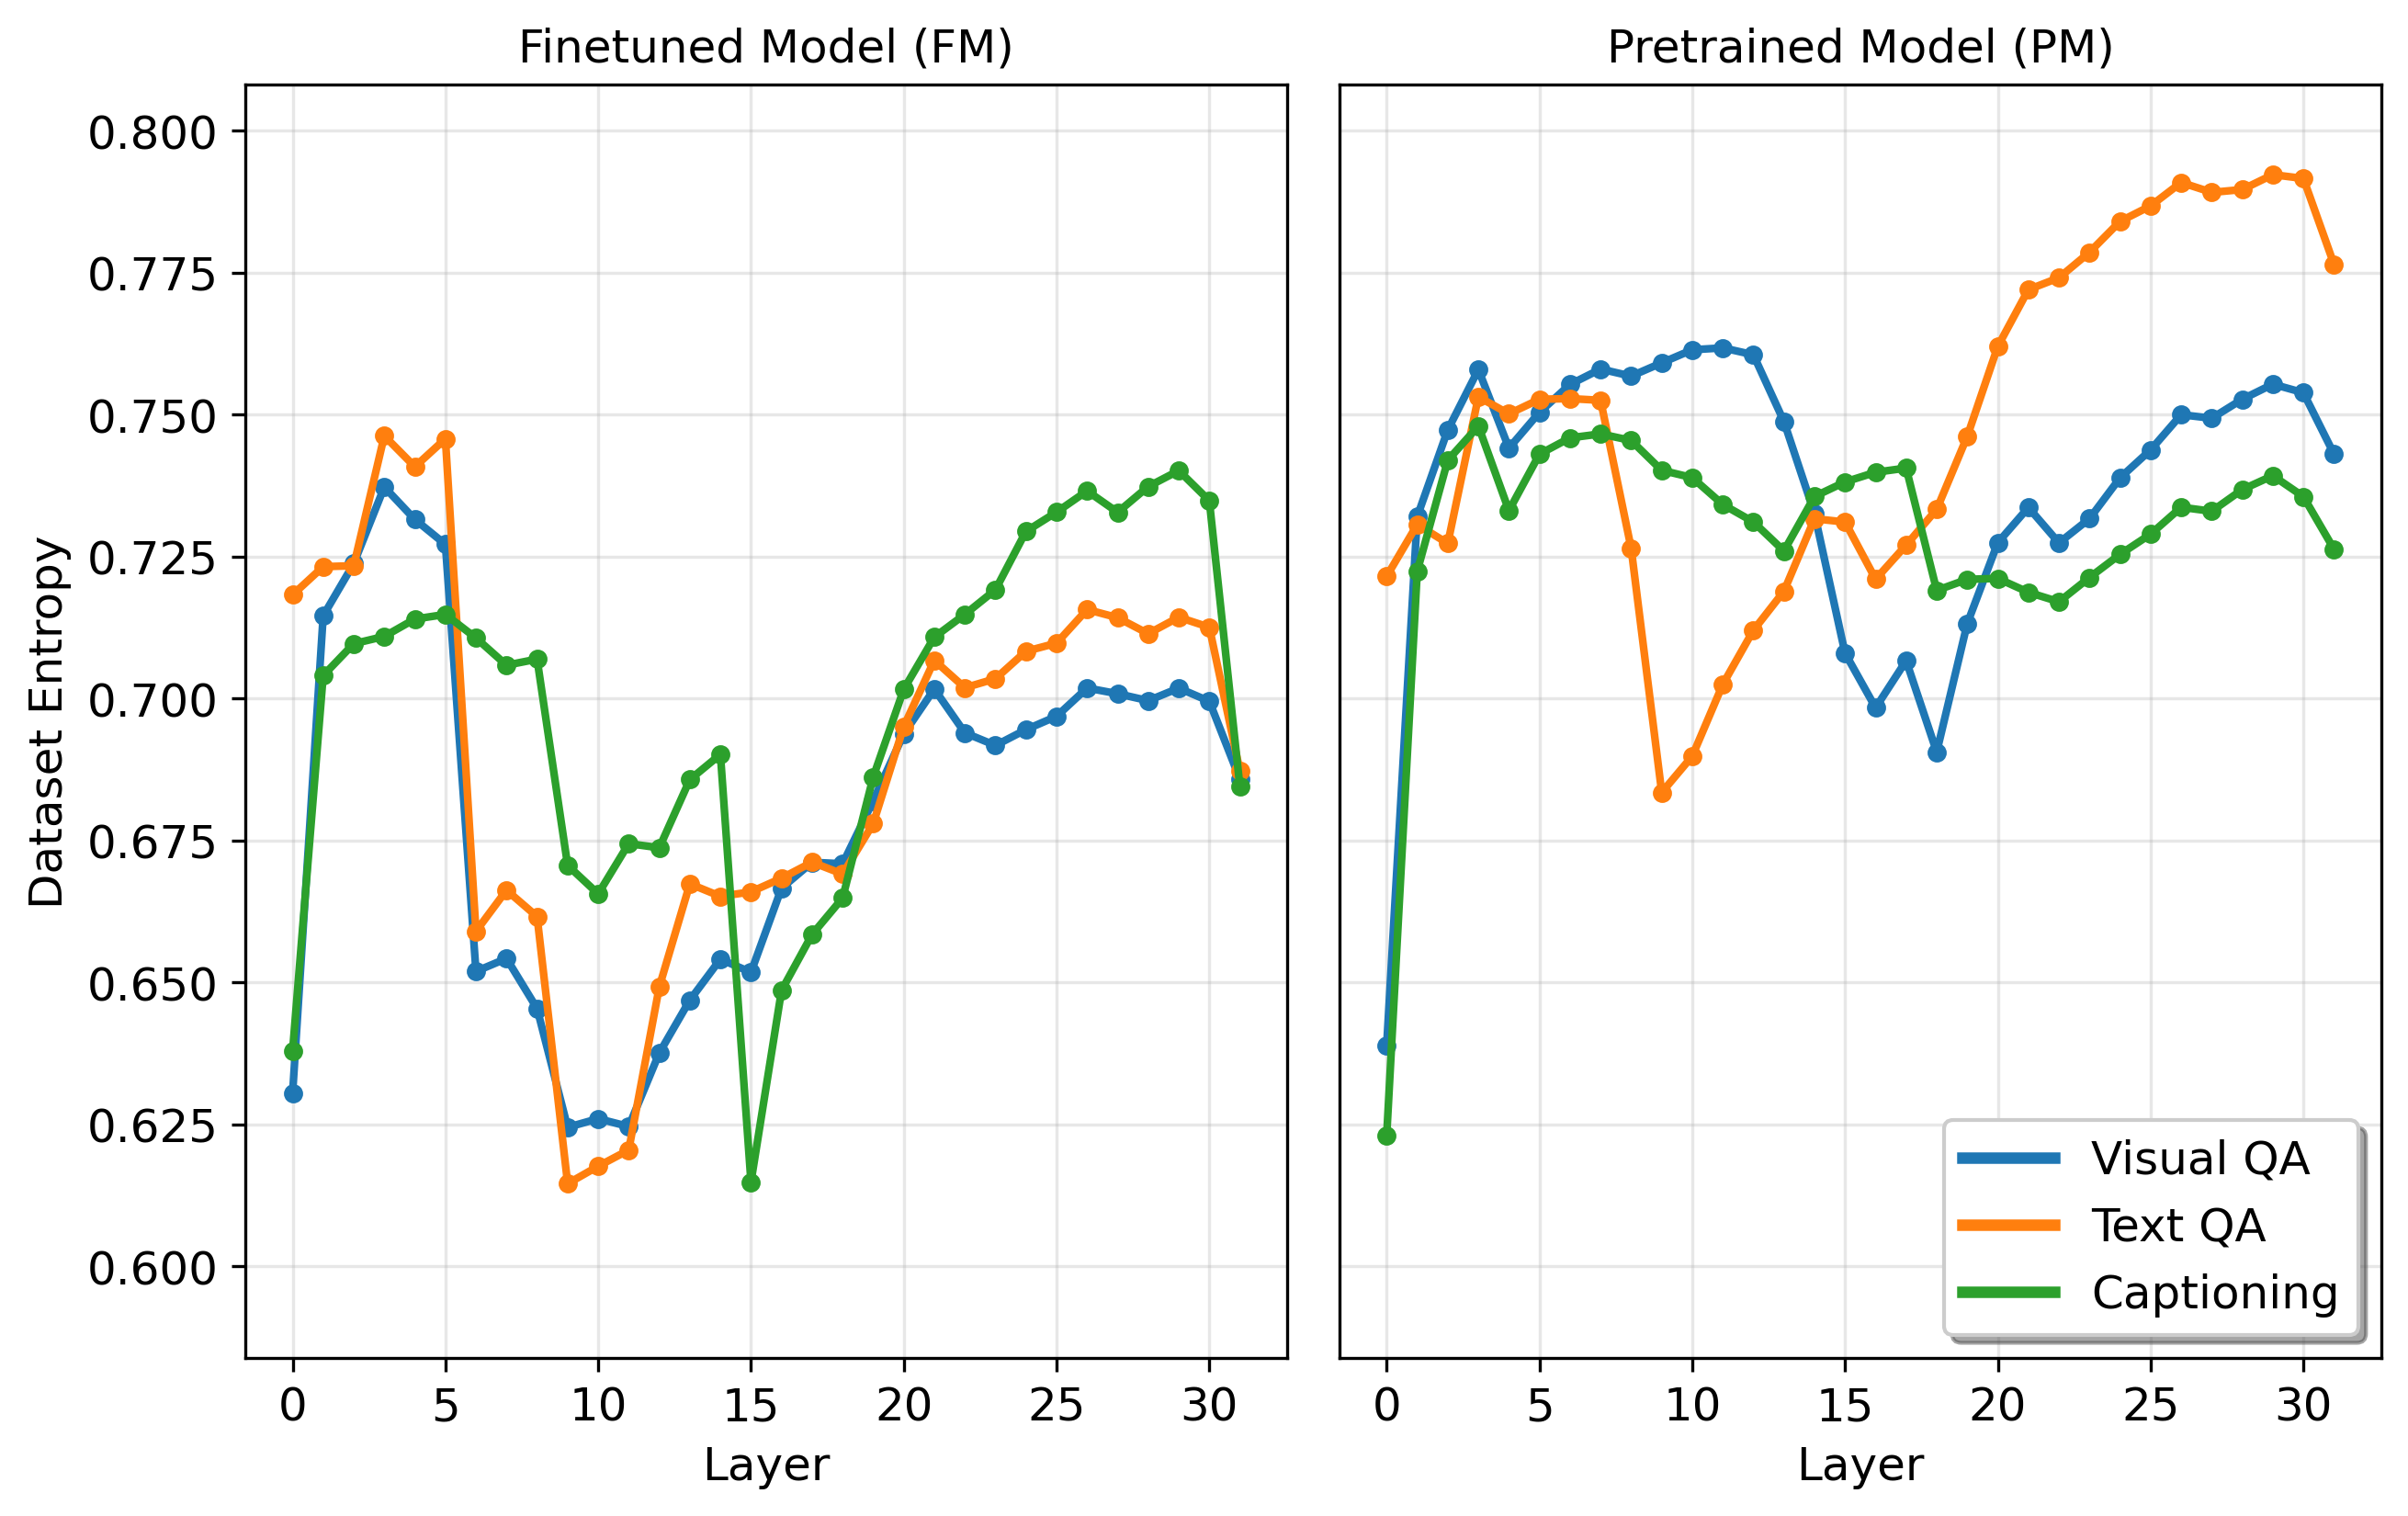
\includegraphics[width=\textwidth]{../images/chapter3/model_data_measures_dataset_entropy_output_layer_last.png}
        \vspace{-0.65cm}
        \caption{}
        \label{fig:dataset_entropy_combined}
    \end{subfigure}
    \begin{subfigure}[t]{0.34\textwidth}
        \centering
        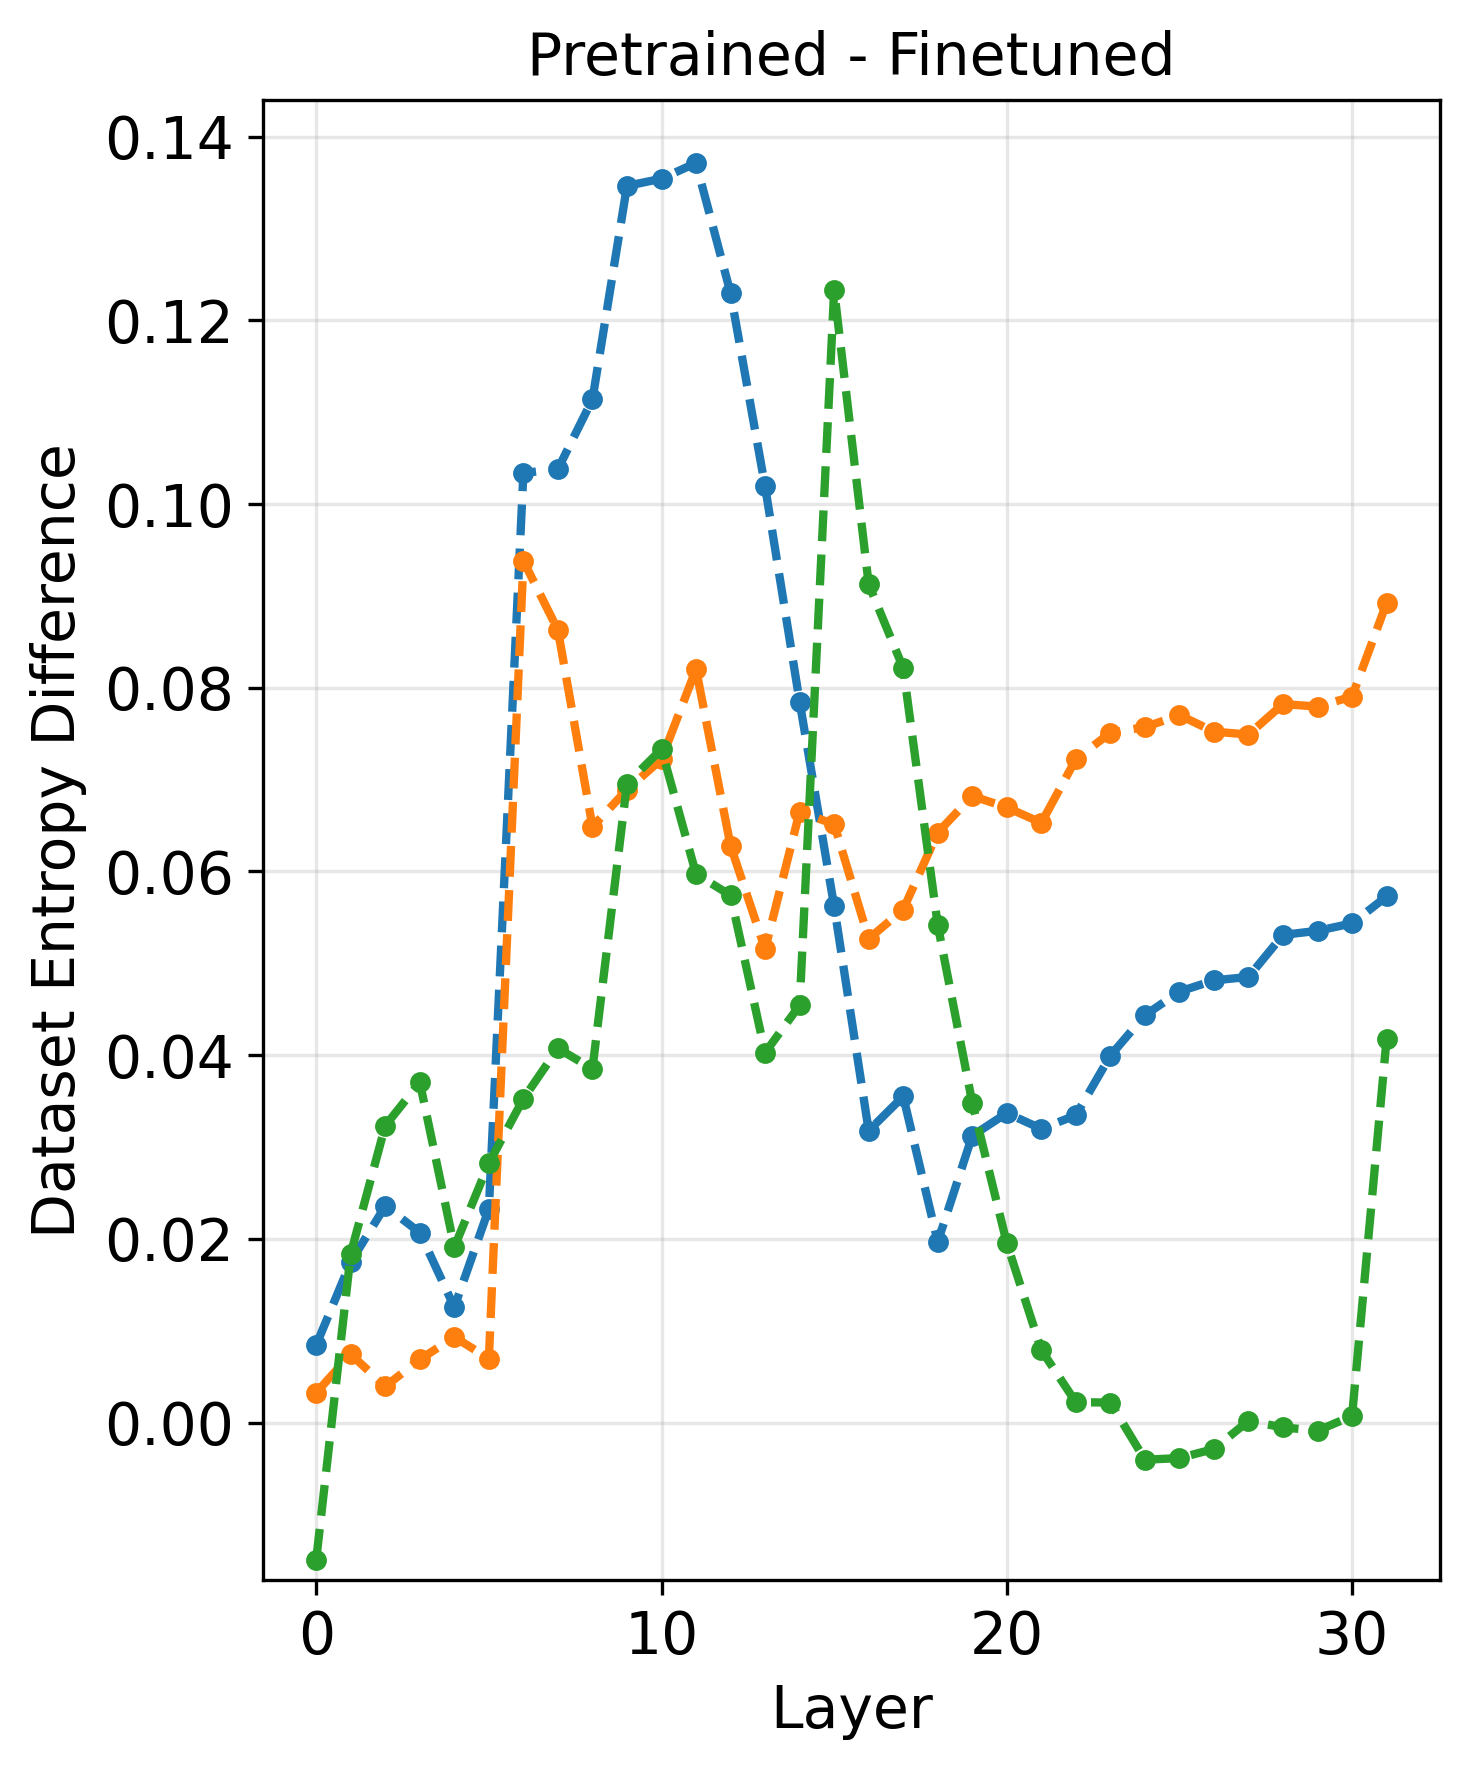
\includegraphics[width=\textwidth]{../images/chapter3/model_data_measures_differences_dataset_entropy.png}
        \vspace{-0.65cm}
        \caption{}
        \label{fig:dataset_entropy_difference}
    \end{subfigure}
    \vspace{-0.3cm}
    \caption{
        Dataset entropy. Similar to Figure~\ref{fig:intrinsic_dimension}. Higher values indicate more diffuse representations, more diverse features and less compact representations.
    }
    \label{fig:dataset_entropy}

\end{figure}

\noindent\textbf{Question Answering with Sliding-Window Layers Patching}

\begin{figure}[H]
    \centering
    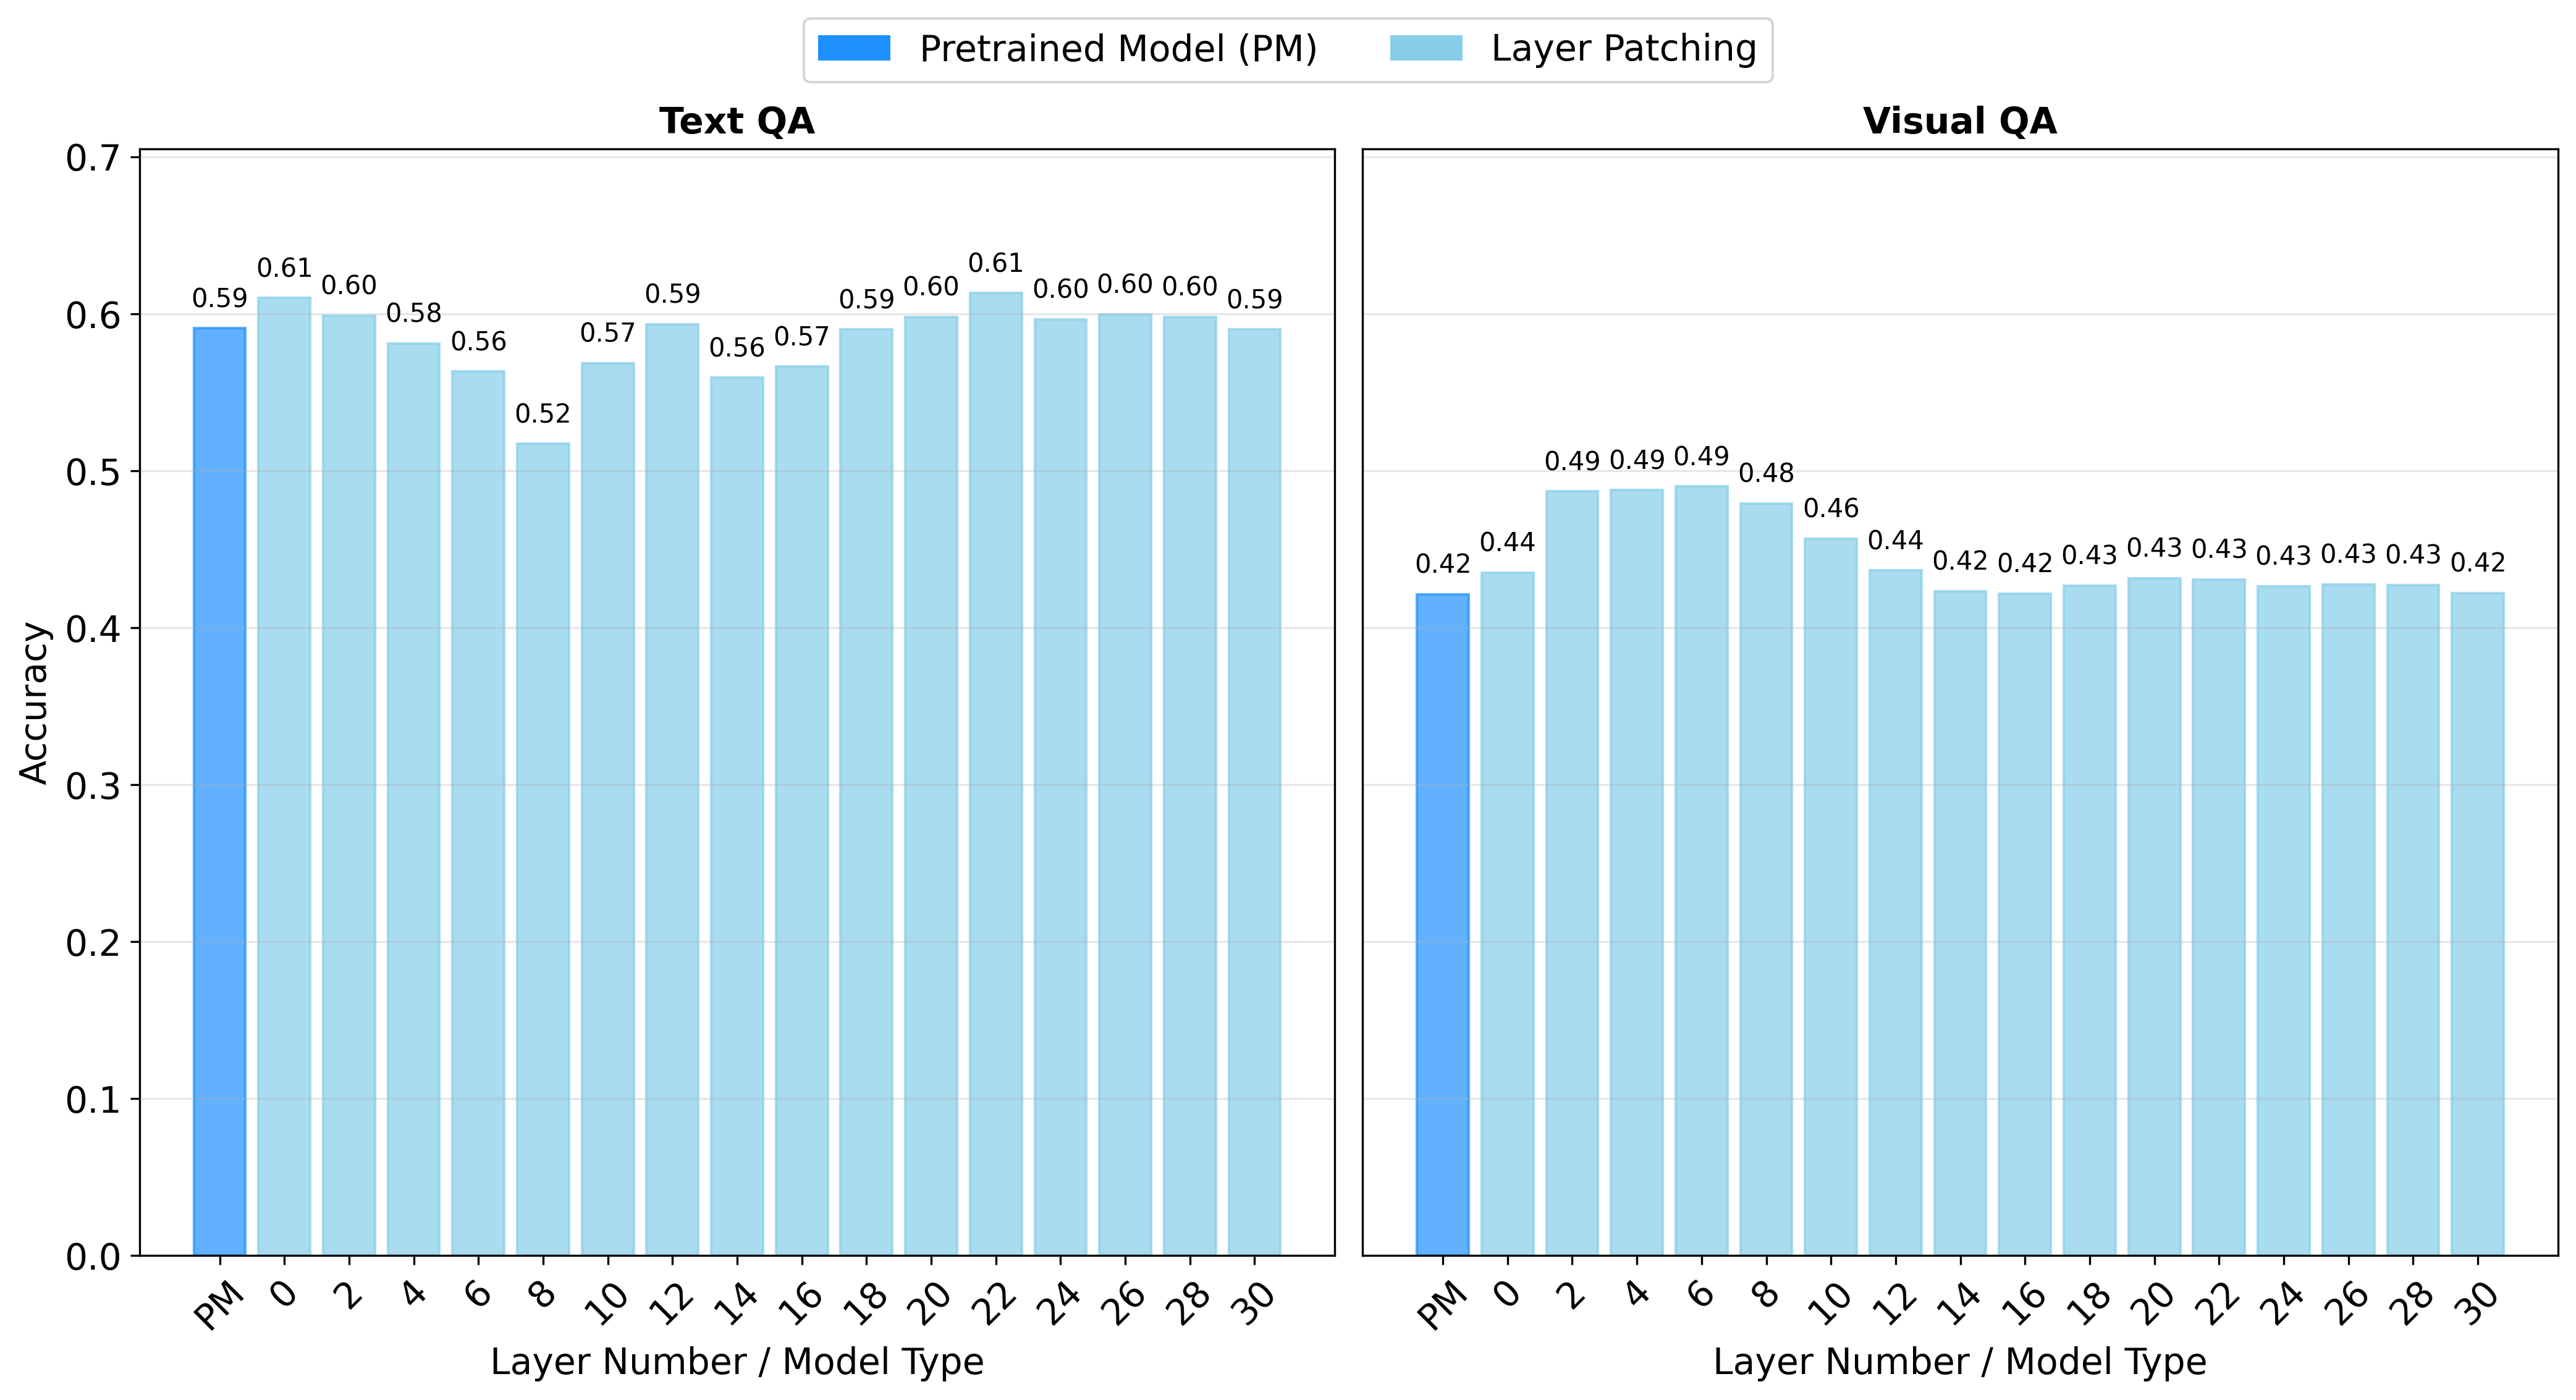
\includegraphics[width=\textwidth]{../images/chapter3/transplanting_layers_qa_benchmarking_sliding_window_ws1_s2.png}
    \caption{
        Sliding-window patching with window size $w=1$ and step $s=2$. The x-axis is $\ell$ (0-indexed; \emph{starting} layer of the patched window). Fine-tuned references: $0.74$ (text QA) and $0.66$ (visual QA). Similar to Figure \ref{fig:accuracy_question_answering_cumulative}.
    }
    \label{fig:accuracy_question_answering_sliding_window}
\end{figure}

\newpage

\noindent\textbf{Image Captioning with Sliding-Window Layers Patching}

\begin{figure}[H]
    \centering
    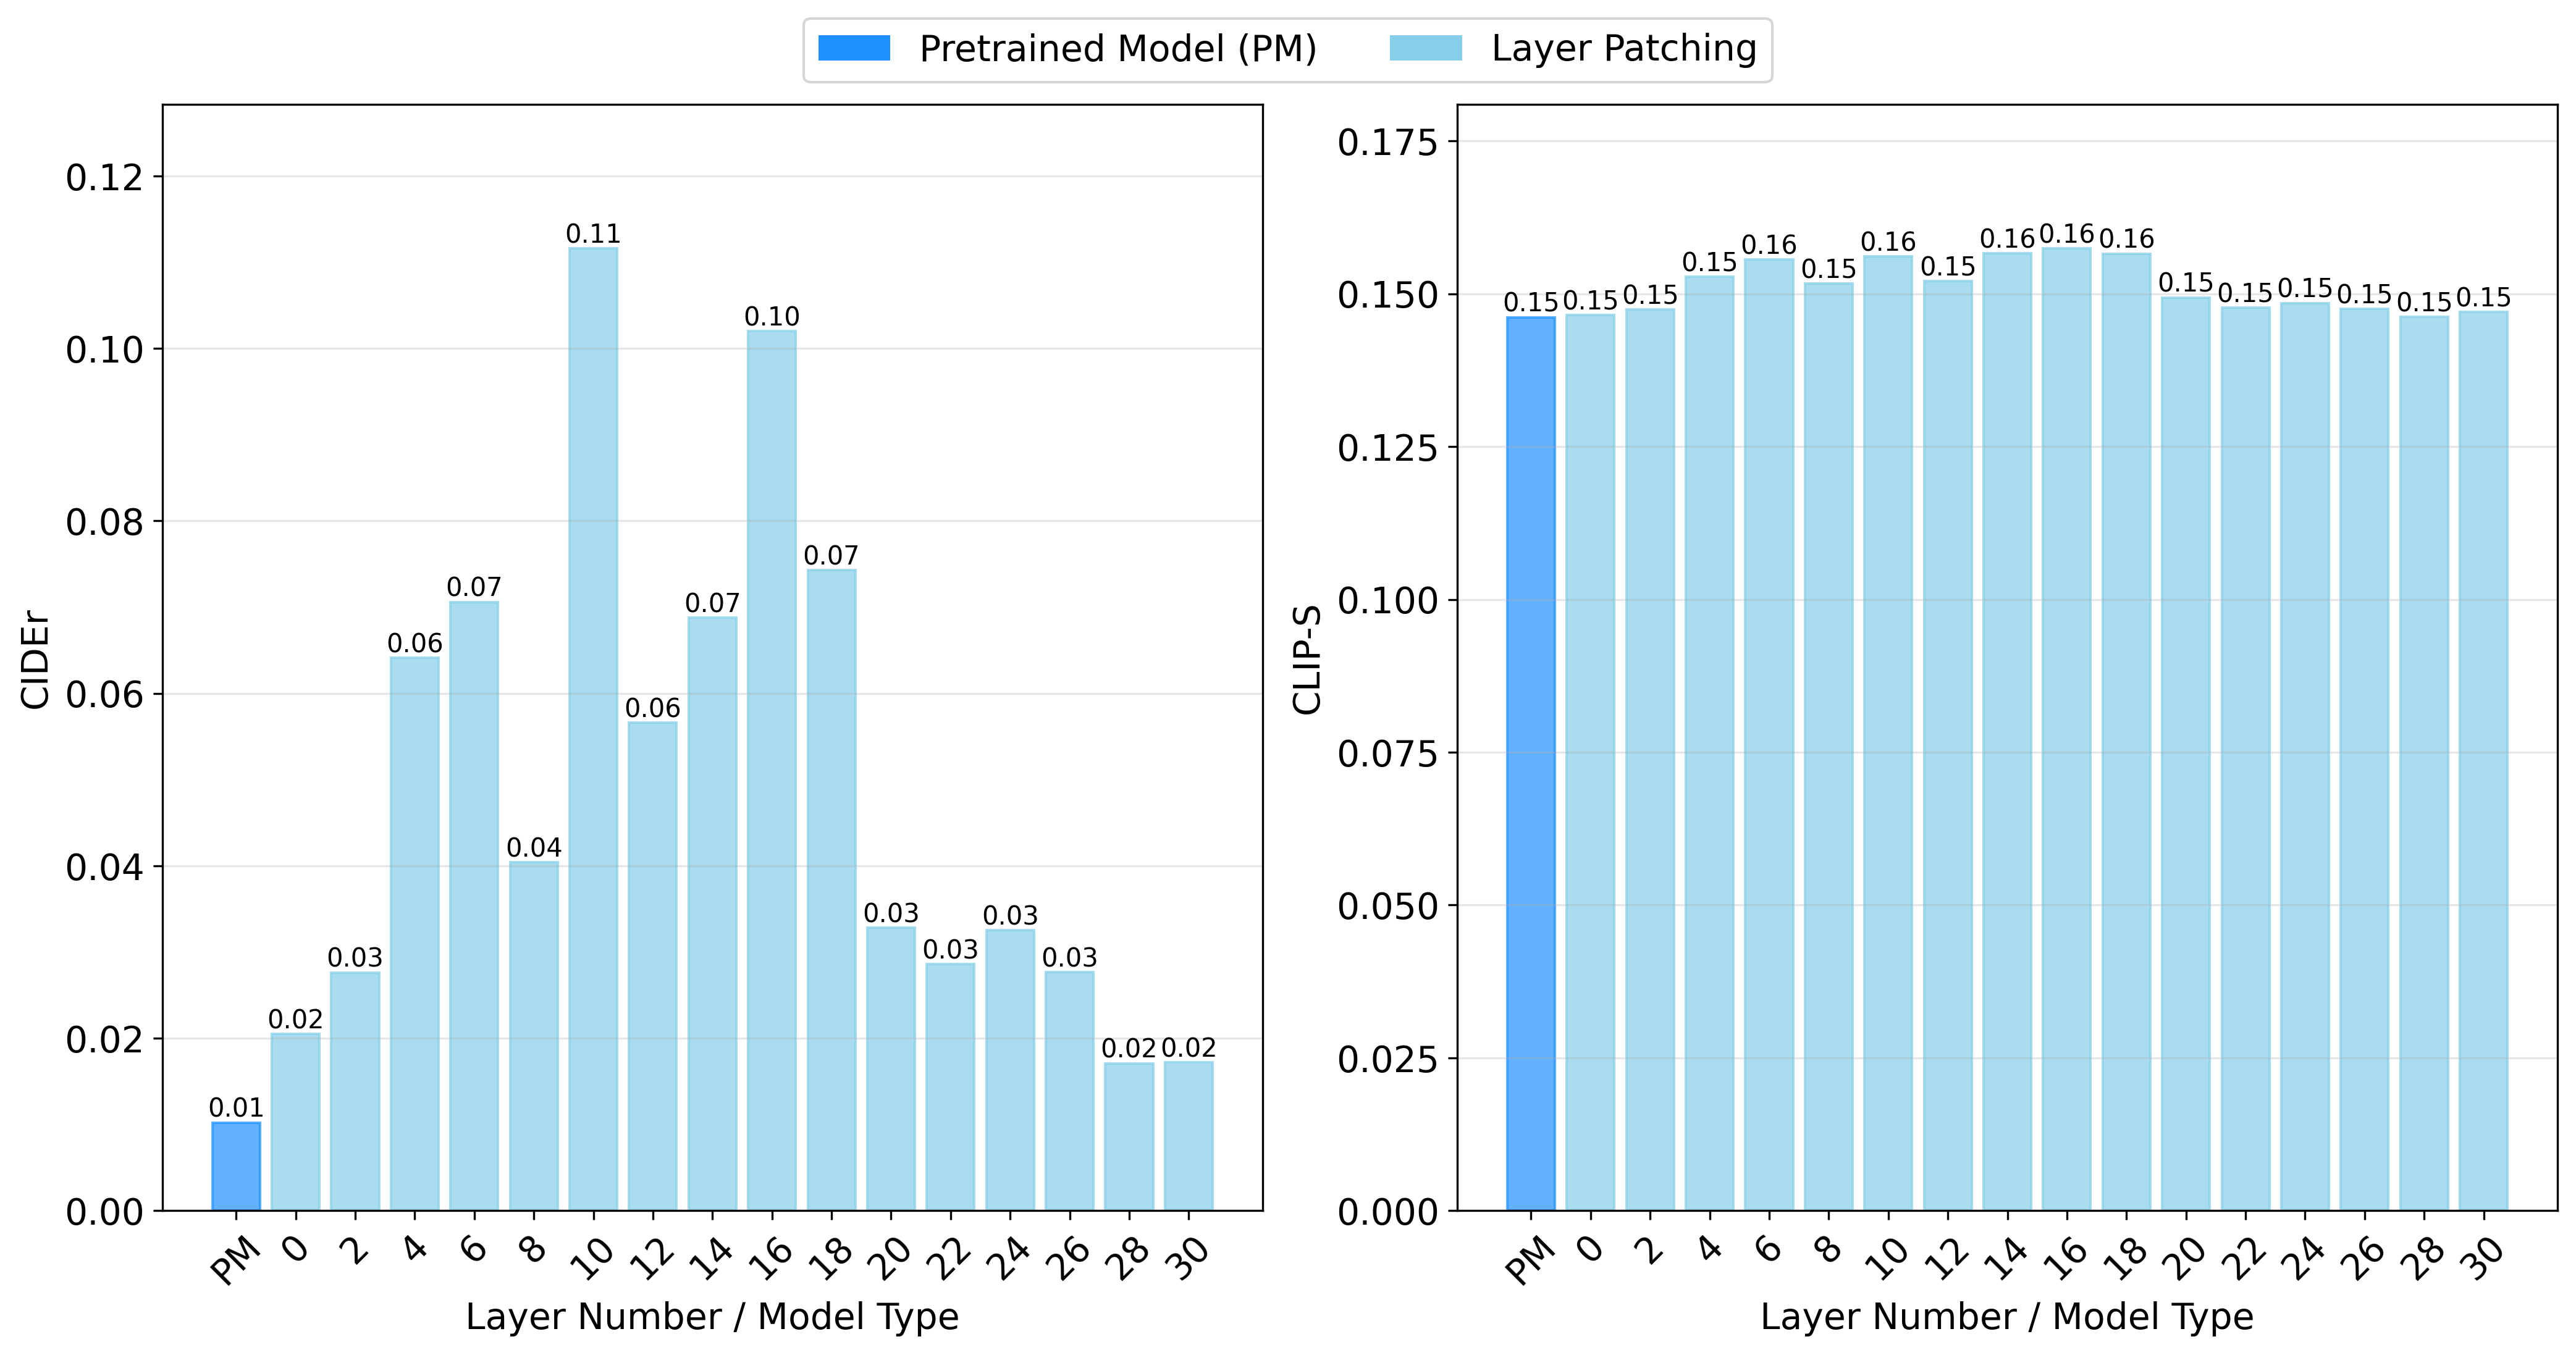
\includegraphics[width=\textwidth]{../images/chapter3/transplanting_layers_caption_benchmarking_combined_sliding_window_tokens100.png}
    \caption{
        Sliding-window patching with $w=1$ (x-axis is the \emph{starting} layer). Fine-tuned references: $0.82$ (CIDEr) and $0.22$ (CLIP-S). Similar to Figure \ref{fig:cider_clip_score_image_captioning_cumulative}.
    }
    \label{fig:cider_clip_score_image_captioning_sliding_window}
\end{figure}